\documentclass[tikz,border=4pt]{standalone}
% Paleta y fuentes compartidas por el libro y las figuras (única fuente de verdad).
\RequirePackage{xcolor}
\definecolor{oxido}{HTML}{B7410E}
\definecolor{cobre}{HTML}{D27D2D}
\definecolor{carbon}{HTML}{2B2B2B}
\definecolor{azul}{HTML}{1F5F8B}
\definecolor{arena}{HTML}{F4EDE4}

\usepackage{fontspec}
\setsansfont{FiraSans}[Extension=.otf,UprightFont=*-Regular,BoldFont=*-Bold,ItalicFont=*-Italic,BoldItalicFont=*-BoldItalic]
\setmonofont{FiraMono}[Extension=.otf,UprightFont=*-Regular,BoldFont=*-Medium]
\usetikzlibrary{positioning,arrows.meta,calc}
\begin{document}
\sffamily\small
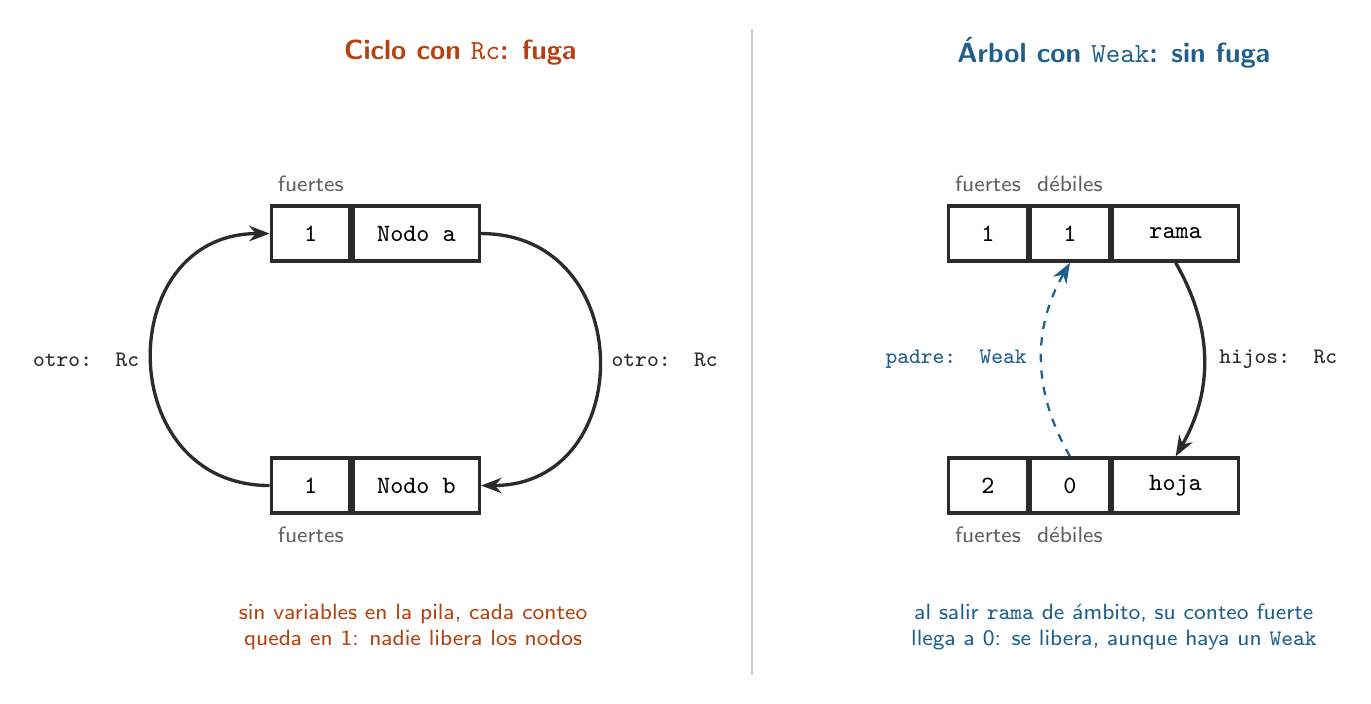
\begin{tikzpicture}[
  celda/.style={draw=carbon,minimum height=7mm,font=\ttfamily\small,fill=white,very thick},
  rotulo/.style={font=\sffamily\footnotesize\color{carbon!75}},
  etiq/.style={font=\sffamily\footnotesize,fill=white,inner sep=2pt},
  >={Stealth[length=2.6mm]}]
  % ---------- Panel izquierdo: ciclo de Rc ----------
  \node[font=\sffamily\bfseries,color=oxido] at (1.9,2.3) {Ciclo con \texttt{Rc}: fuga};
  \node[celda,minimum width=10mm] (af) at (0,0) {1};
  \node[celda,minimum width=16mm,anchor=west] (an) at (af.east) {Nodo a};
  \node[rotulo,above=1pt of af] {fuertes};
  \node[celda,minimum width=10mm] (bf) at (0,-3.2) {1};
  \node[celda,minimum width=16mm,anchor=west] (bn) at (bf.east) {Nodo b};
  \node[rotulo,below=1pt of bf] {fuertes};
  \draw[->,very thick,carbon] (an.east) to[out=0,in=0,looseness=1.6]
    node[etiq,right=2pt] {\texttt{otro: Rc}} (bn.east);
  \draw[->,very thick,carbon] (bf.west) to[out=180,in=180,looseness=1.6]
    node[etiq,left=2pt] {\texttt{otro: Rc}} (af.west);
  \node[font=\sffamily\footnotesize,align=center,text=oxido] at (1.3,-5.0)
    {sin variables en la pila, cada conteo\\queda en 1: nadie libera los nodos};
  % ---------- Panel derecho: árbol con Weak ----------
  \begin{scope}[xshift=8.6cm]
  \node[font=\sffamily\bfseries,color=azul] at (1.6,2.3) {Árbol con \texttt{Weak}: sin fuga};
  \node[celda,minimum width=10mm] (rf) at (0,0) {1};
  \node[celda,minimum width=10mm,anchor=west] (rd) at (rf.east) {1};
  \node[celda,minimum width=16mm,anchor=west] (rn) at (rd.east) {rama};
  \node[rotulo,above=1pt of rf] {fuertes};
  \node[rotulo,above=1pt of rd] {débiles};
  \node[celda,minimum width=10mm] (hf) at (0,-3.2) {2};
  \node[celda,minimum width=10mm,anchor=west] (hd) at (hf.east) {0};
  \node[celda,minimum width=16mm,anchor=west] (hn) at (hd.east) {hoja};
  \node[rotulo,below=1pt of hf] {fuertes};
  \node[rotulo,below=1pt of hd] {débiles};
  \draw[->,very thick,carbon] (rn.south) to[out=-60,in=60]
    node[etiq,right=3pt] {\texttt{hijos: Rc}} (hn.north);
  \draw[->,thick,azul,dashed] (hd.north) to[out=120,in=-120]
    node[etiq,left=3pt,text=azul] {\texttt{padre: Weak}} (rd.south);
  \node[font=\sffamily\footnotesize,align=center,text=azul] at (1.6,-5.0)
    {al salir \texttt{rama} de ámbito, su conteo fuerte\\llega a 0: se libera, aunque haya un \texttt{Weak}};
  \end{scope}
  \draw[carbon!25,thick] (5.6,2.6) -- (5.6,-5.6);
\end{tikzpicture}
\end{document}
